\chapter{Architettura della soluzione - Tecnologie}
\section{Pattern MVC}
Per lo sviluppo della web app ho utilizzato il pattern MVC.
Il Model-View-Controller è un pattern utilizzato per dividere il codice in blocchi che svolgono funzionalità distinte.

Esso è costituito da tre componenti principali\cite{patternMVC} (Figura \ref{fig:pattern-mvc}):
\begin{itemize}
    \item Model: si occupa di accedere ai dati necessari alla logica implementata nell'applicazione. In particolare nella nostra web app all'interno dei model avremo la classe Postit.
    \item View: si occupano di creare l'interfaccia utilizzabile dall'utente, mostrando i dati richiesti da quest'ultimo. Nel nostro caso la view si occuperà di visualizzare, la pagina di login e tutti i postit nella homepage.
    \item Controller: si occupano di implementare la vera logica dell'applicazione utilizzando i due componenti precedenti, ricevendo gli input dell'utente, gestendo i model per la ricerca dei dati e la creazione delle view da restituire all'utente. Nel nostro caso usiamo due controller: uno per la gestione del login e uno per la gestione dei postit.
\end{itemize}
\begin{figure}[h]
    \centering
    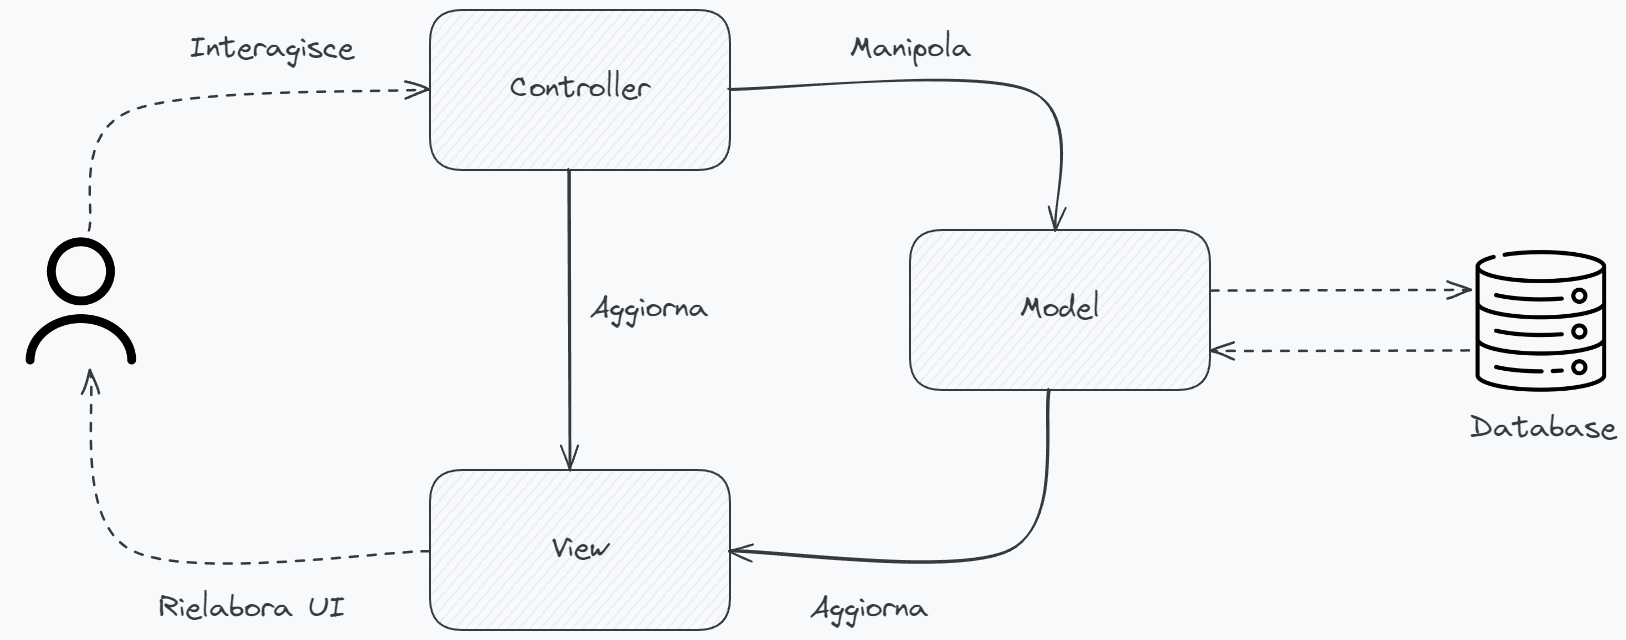
\includegraphics[width=1.0\textwidth]{images/pattern mvc.png}
    \caption{Funzionamento pattern MVC}
    \label{fig:pattern-mvc}
\end{figure}

\newpage
\section{Back-end: Tecnologie utilizzate}
Per l'implementazione del back-end ho utilizzato diverse tecnologie:
\begin{itemize}
    \item Java Spring Boot: per la gestione della logica lato server;
    \item Maven: build automation tool;
    \item Docker: per dockerizzare in un container il DB di PostgreSQL;
    \item Bcrypt: algoritmo di hashing di password;
\end{itemize}


\subsection{Spring}
Spring è un framework di Java che viene utilizzato per la creazione di applicazioni autonome, adatte ad ambienti di produzione che vengono eseguite su Java Virtual Machine.\\
Spring Boot è uno strumento che semplifica e velocizza lo sviluppo delle applicazioni web che usano Spring.
Spring fornisce una funzione di dependency-injection, che consente agli oggetti di definire le proprie dipendenze che successivamente il container Spring provvederà ad inserire. Ciò garantisce la possibilità di creare applicazioni modulari.
Dato che Spring richiede un notevole dispendio di tempo e competenze per configurare, impostare e implementare applicazioni Spring, Spring Boot riduce questo sforzo usando tre funzionalità\cite{spring}:
\begin{itemize}
    \item Configurazione automatica: le applicazioni vengono inizializzate con dipendenze preimpostate in modo tale da non doverle configurare manualmente. Grazie alla configurazione automatica, Spring Boot è in grado di configurare sia le impostazioni di Spring sia i pacchetti di terze parti. Ciò garantisce la possibilità di iniziare velocemente a sviluppare le applicazioni, riducendo errori umani.
    \item Approccio categorico per le dipendenze: Spring è in grado di scegliere i pacchetti da installare e i valori predefiniti da utilizzare evitando allo sviluppatore la perdita di tempo nel prendere tutte queste decisioni. In particolar modo durante la creazione del progetto è possibile selezionare già le dipendenze necessarie, grazie allo Spring Boot Initializr compilando semplicemente un modulo web (Figura \ref{fig:spring-initializr}). Ad esempio per la creazione di un'applicazione web è possibile selezionare "Spring Web", per garantire la sicurezza è possibile selezionare "Spring Security", ecc...
    \item Applicazioni autonome: Spring Boot consente di creare applicazioni autonome che vengono eseguite automaticamente integrando un server web come ad esempio Tomcat nell'applicazione durante il processo di inizializzazione senza dover far affidamento su un server web esterno.
\end{itemize}
\newpage
\begin{figure}[h]
    \centering
    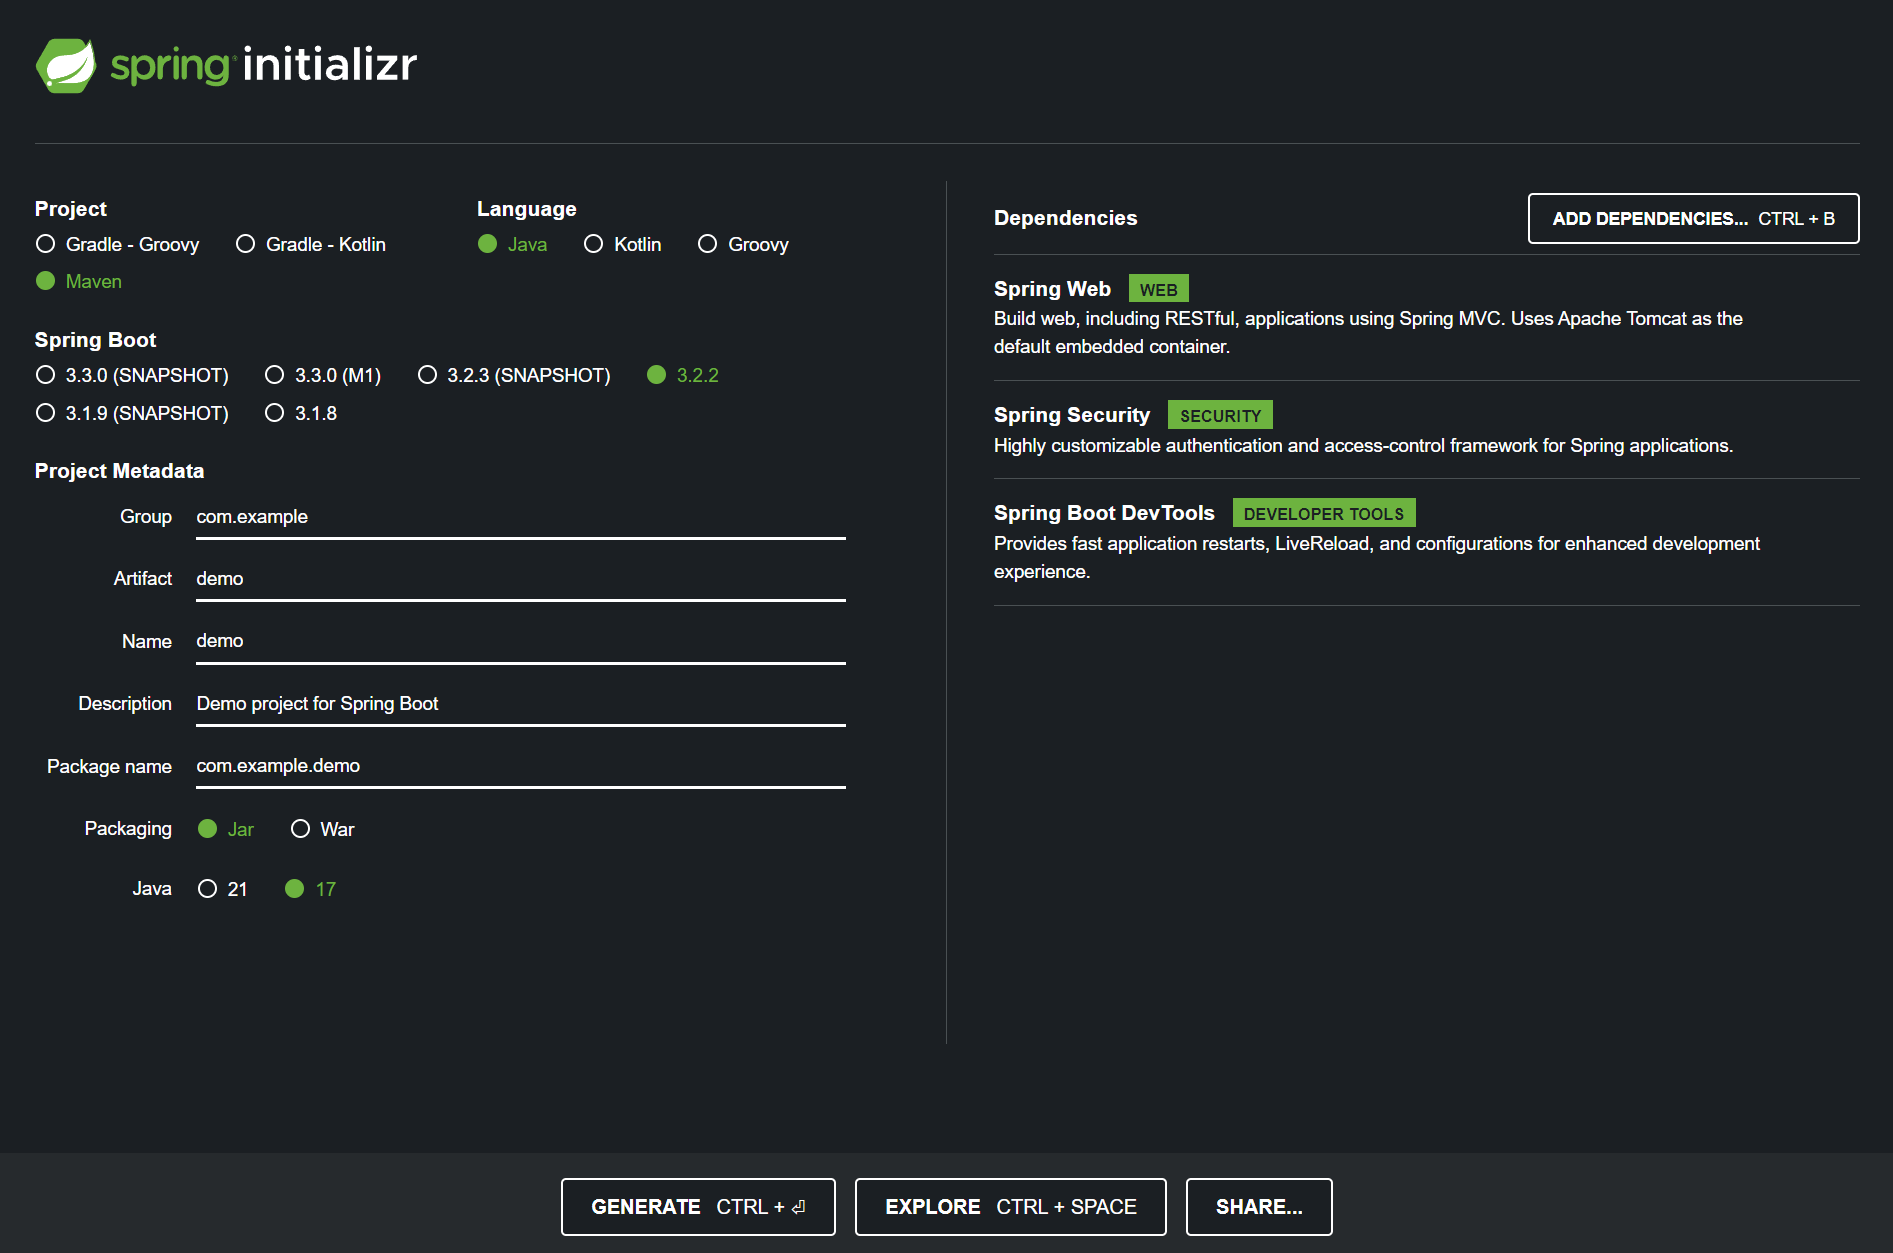
\includegraphics[width=1.0\textwidth]{images/spring initializr.png}
    \caption{Modulo web Spring Initializr}
    \label{fig:spring-initializr}
\end{figure}
\newpage

\subsection{Maven}
Apache Maven è uno strumento di automazione build utilizzato per i progetti Java.
Rende più facile gestire e mantenere grandi progetti fornendo una struttura coerente e una serie di convenzioni su come organizzare il progetto (Figura \ref{fig:organizzazione-progetto}), aiutando gli sviluppatori ad automatizzare il processo di build, test e distribuzione del software.

Una delle caratteristiche di Maven è la capacità di gestire le dipendenze, tenendo traccia di tutte le librerie e altre dipendenze di cui un progetto ha bisogno, scaricandole automaticamente.
Ciò aiuta gli sviluppatori senza il bisogno che debbano scaricare e gestire manualmente le dipendenze.\cite{maven}
\begin{figure}[h]
    \centering
    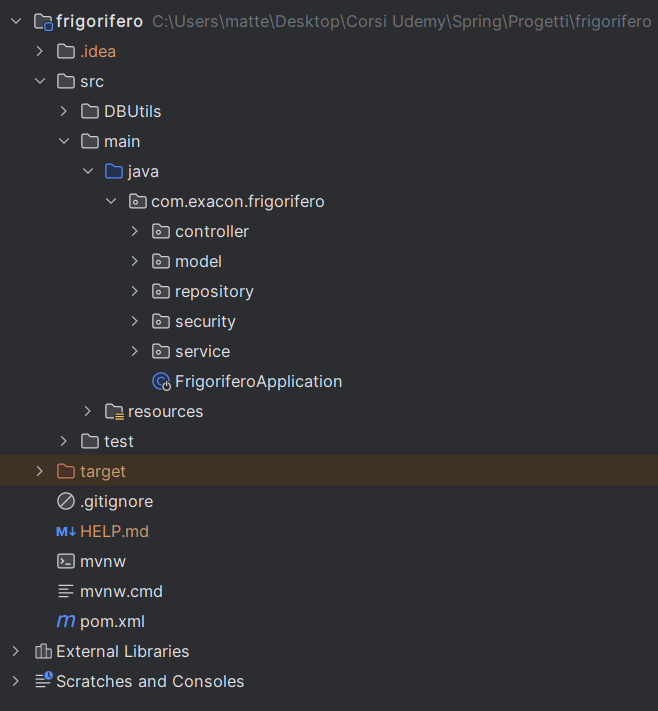
\includegraphics[scale=0.8]{images/esempio struttura progetto maven.png}
    \caption{Struttura del progetto postit-app utilizzando Maven}
    \label{fig:organizzazione-progetto}
\end{figure}

\newpage
\subsubsection{Project Object Model}
Per la gestione delle dipendenze del progetto, i plugin e la configurazione di build, Maven utilizza un file XML chiamato pom.xml (project object model).

\begin{lstlisting}[language = xml,  basicstyle=\tiny, caption={Esempio di pom.xml, nel quale sono state aggiunte le dipendenze web e database.}, captionpos=b]
<?xml version="1.0" encoding="UTF-8"?>
<project xmlns="http://maven.apache.org/POM/4.0.0" xmlns:xsi="http://www.w3.org/2001/XMLSchema-instance"
	xsi:schemaLocation="http://maven.apache.org/POM/4.0.0 https://maven.apache.org/xsd/maven-4.0.0.xsd">
	<modelVersion>4.0.0</modelVersion>
	
	<parent>
		<groupId>org.springframework.boot</groupId>
		<artifactId>spring-boot-starter-parent</artifactId>
		<version>3.2.2</version>
		<relativePath/> <!-- lookup parent from repository -->
	</parent>
	<groupId>com.example</groupId>
	<artifactId>demo</artifactId>
	<version>0.0.1-SNAPSHOT</version>
	<name>demo</name>
	<description>Demo project for Spring Boot</description>
	<properties>
		<java.version>17</java.version>
	</properties>
	
	<dependencies>
		
		<dependency>
			<groupId>org.springframework.boot</groupId>
			<artifactId>spring-boot-starter-web</artifactId>
		</dependency>

		<dependency>
			<groupId>org.postgresql</groupId>
			<artifactId>postgresql</artifactId>
			<scope>runtime</scope>
		</dependency>
		
		<dependency>
			<groupId>org.springframework.boot</groupId>
			<artifactId>spring-boot-starter-test</artifactId>
			<scope>test</scope>
		</dependency>
		
	</dependencies>

	<build>
		<plugins>
			<plugin>
				<groupId>org.springframework.boot</groupId>
				<artifactId>spring-boot-maven-plugin</artifactId>
			</plugin>
		</plugins>
	</build>

</project>

\end{lstlisting}

\newpage

\subsection{Docker}
Docker è una piattaforma open source che consente agli sviluppatori di creare, implementare, eseguire, aggiornare e gestire container, i quali sono delle unità eseguibili di software in cui viene impacchettato il codice applicativo, insieme alle sue librerie e dipendenze in modo da poter essere eseguito ovunque.
I container sono piccoli, veloci e portabili perché, diversamente da una Virtual Machine (VM), non hanno bisogno di includere un sistema operativo guest in ogni istanza, ma possono invece sfruttare le funzioni e le risorse del sistema operativo host. \cite{docker}
\subsubsection{Differenza tra container e virtual machine}
Ogni VM contiene un sistema operativo guest, una copia virtuale dell'hardware di cui il sistema operativo ha bisogno per essere eseguito, insieme a un'applicazione e alle relative librerie e dipendenze associate.
I container, a differenza delle VM, virtualizzano il sistema operativo, in modo che ogni singolo container includa solo l'applicazione e le relative librerie e dipendenze.\cite{container}
L'utilizzo dei container porta diversi vantaggi:
\begin{itemize}
    \item Leggero: i container condividono il kernel del sistema operativo della macchina, eliminando la necessità di un'istanza del sistema operativo completa per ogni applicazione e rendendo i file container piccoli e poco gravosi sulle risorse. Ciò garantisce un'esecuzione più rapida.
    \item Portabile: i container portano con loro tutte le loro dipendenze, in modo tale che il software debba essere scritto una sola volta e eseguito in diversi ambienti senza doverlo riconfigurare ogni volta.
\end{itemize}

\subsubsection{Creazione database in un container}
Per gestione del database della web app ho inserito in un container il database di PostgreSQL.
Per inserire il db in un container ho eseguito all'interno del terminale il seguente comando:
\\
\begin{lstlisting}[language=xml]
docker run --name postit-app-db ^
 -e POSTGRES_USER=utente ^
 -e POSTGRES_DB=postit-app-db ^
 -e POSTGRES_PASSWORD=password ^
 -e PGDATA=/var/lib/postgresql/data/postitData ^
 -p 5434:5432 ^
 -v C:\Docker_Data:/var/lib/postgresql/data ^
 postgres:14.1-alpine
\end{lstlisting}
\newpage
\subsubsection{Docker Desktop}
Tramite l'utilizzo dell'applicazione Docker Desktop, è possibile gestire i container ed eseguirli.
In Figura \ref{fig:docker-desktop} è possibile vedere che il container "postit-app-db" è in esecuzione.
\begin{figure}[h]
    \centering
    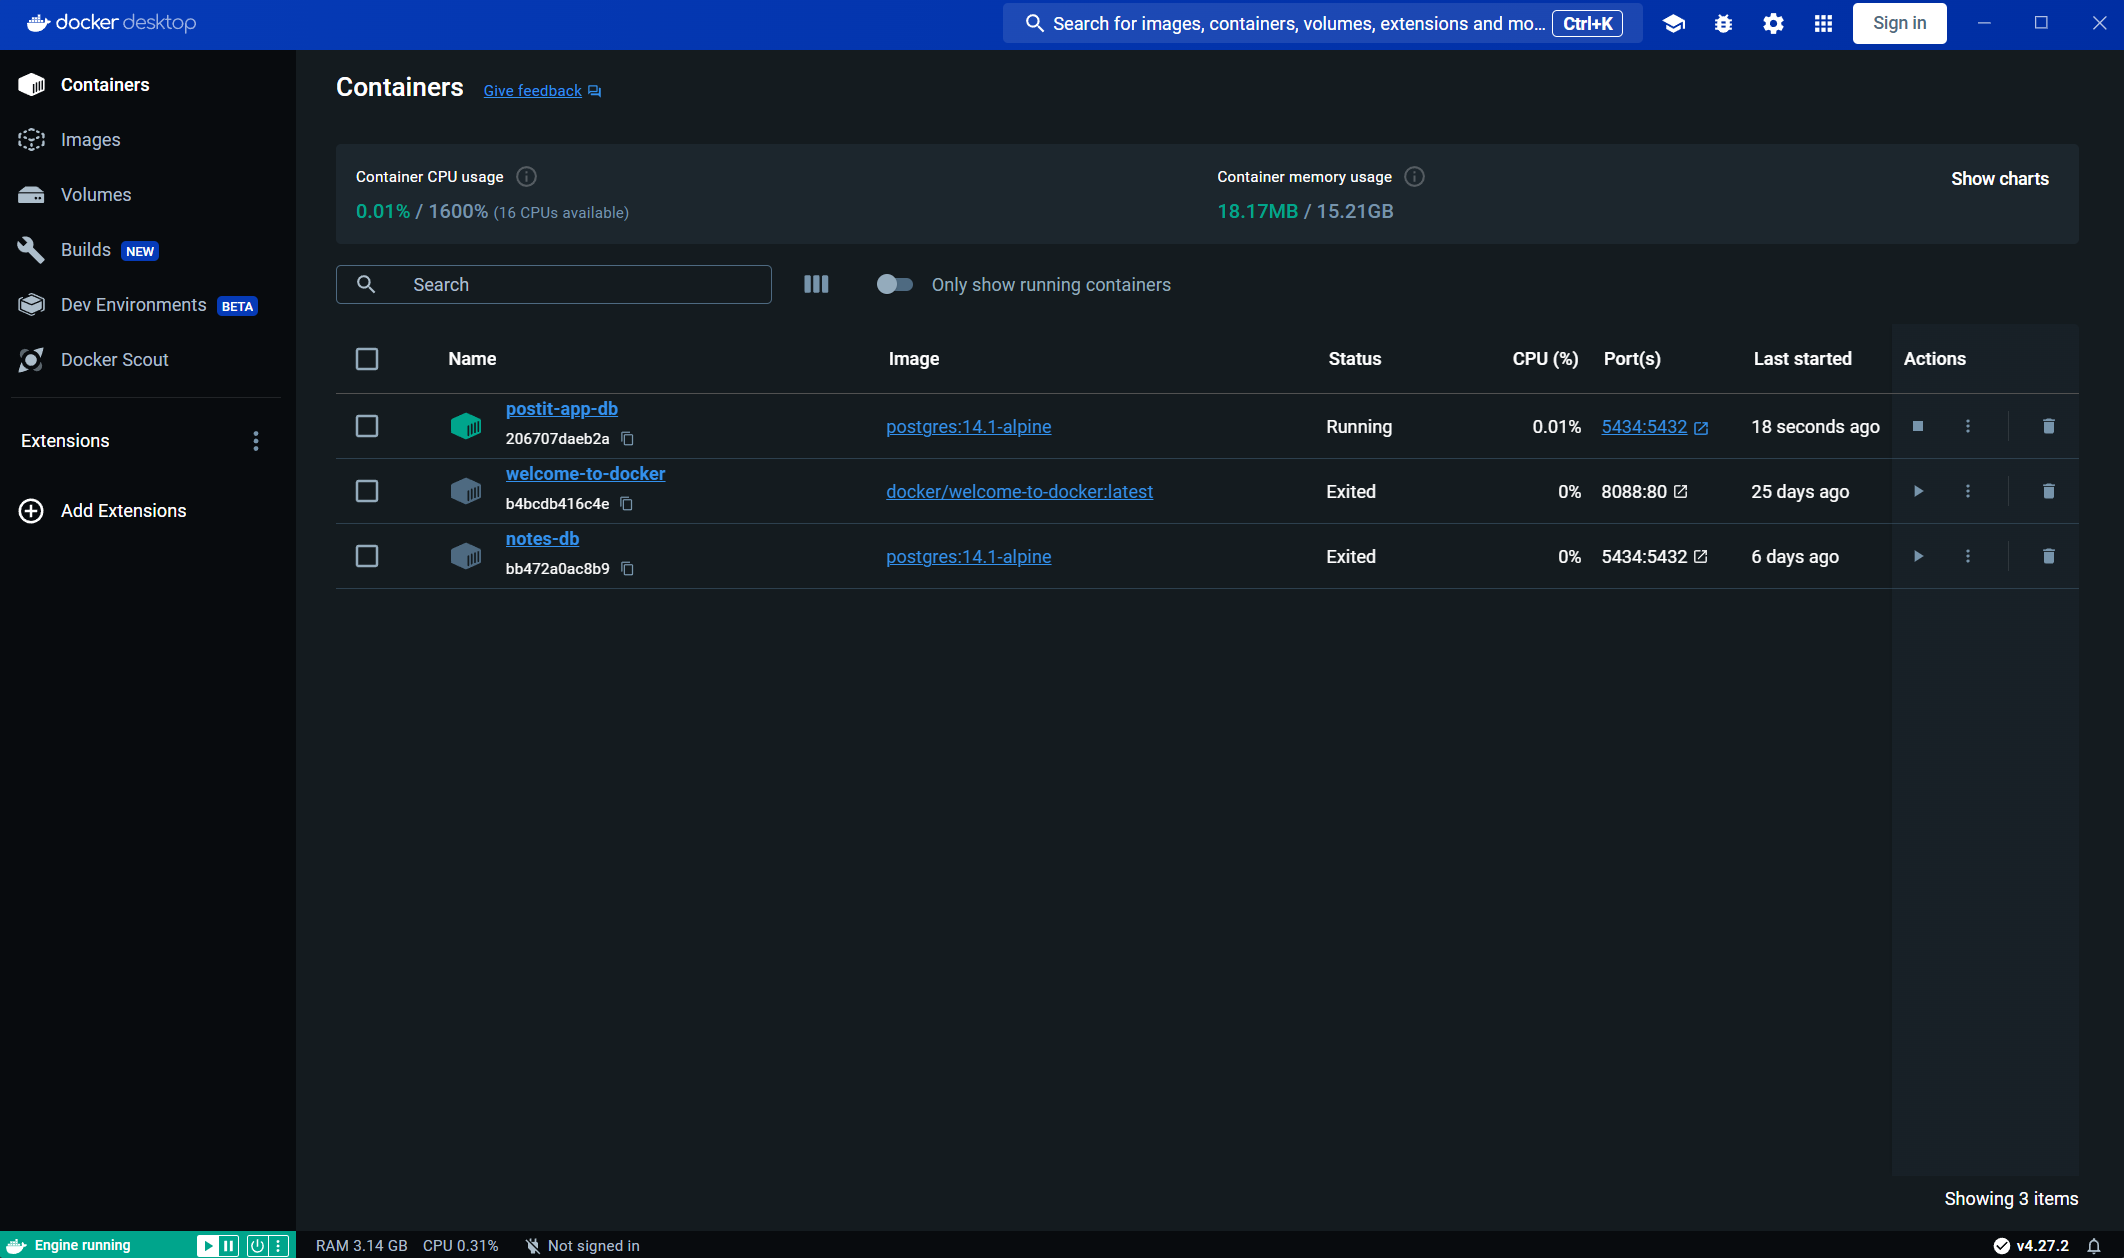
\includegraphics[width=1.0\textwidth]{images/interfaccia docker desktop.png}
    \caption{Interfaccia di Docker Desktop}
    \label{fig:docker-desktop}
\end{figure}
\newpage
\subsection{JPA - Hibernate}

\subsubsection{JPA}
Jakarta Persistent API (JPA) è un interfaccia di programmazione che consente agli sviluppatori di lavorare con i database utilizzando Java.
Viene utilizzato per recuperare e aggiornare i dati in un database.
JPA si basa sulla tecnica di programmazione ORM (Object-Relational Mapping) e può essere implementato da vari framework ORM come Hibernate (Figura \ref{fig:jpa-hibernate}) ed essere anche usato in combinazione con tecnologie Java come Spring.\cite{jpa}

\subsubsection{Hibernate}
Hibernate ORM è un framework Java utilizzato per mappare modelli di dominio orientati agli oggetti su un database relazionale (Figura \ref{fig:hibernate}).
Sostanzialmente Hibernate viene utilizzato per rendere persistenti i dati dall'ambiente Java al database.
Hibernate implementa le specifiche JPA per la persistenza dei dati\footnote{In informatica, il concetto di persistenza si riferisce alla caratteristica dei dati di un programma di sopravvivere all'esecuzione del programma stesso che li ha creati.
La persistenza si riferisce in particolare alla possibilità di far sopravvivere delle strutture dati all'esecuzione di un singolo programma. In ogni caso questa possibilità è raggiunta salvando i dati in uno storage non volatile, come su un file system o su un database. \cite{persistenza}}.\cite{hibernate}
\\
\begin{figure}[h]
    \centering
    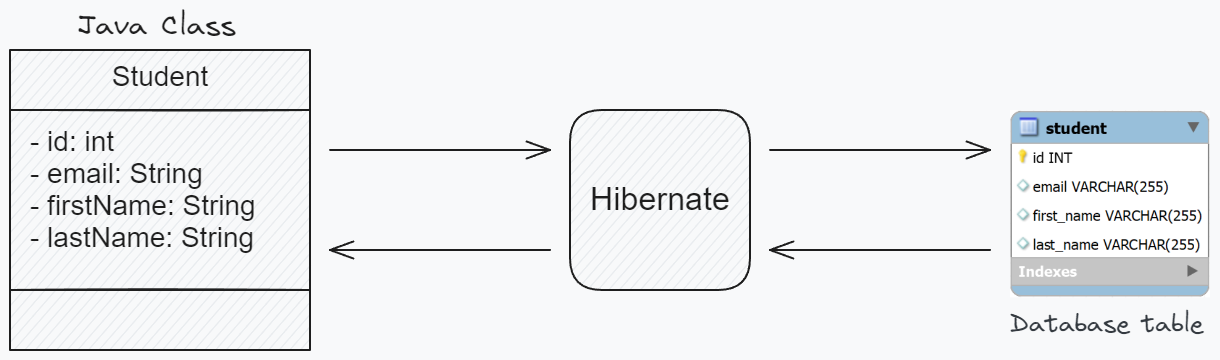
\includegraphics[width=1.0\textwidth]{images/hibernate.png}
    \caption{Funzionamento di Hibernate}
    \label{fig:hibernate}
\end{figure}

\subsubsection{JDBC}
JDBC (Java Database Connectivity) è un'API che permette di eseguire query SQL all'interno di un'applicazione Java, consentendo a queste ultime di connettersi e interrogare dei database come PostgreSQL o MySQL.\cite{jdbc}

\newpage
\subsubsection{Object-Relational Mapping}
L'Object-Relational Mapping (ORM) è una tecnica di programmazione utilizzata per memorizzare, richiamare, aggiornare ed eliminare dati da un database all'interno di programmi object-oriented solitamente scritti utilizzando linguaggi di programmazione orientata agli oggetti (OOP), come Java o C\#.
L'ORM si applica ai database relazionali, conosciuti come RDBMS (Relational Database Management System), e si occupa di convertire e tradurre tutti i dati che non potrebbero altrimenti coesistere tra database e linguaggi OOP.\cite{orm}
\\
\begin{figure}[h]
    \centering
    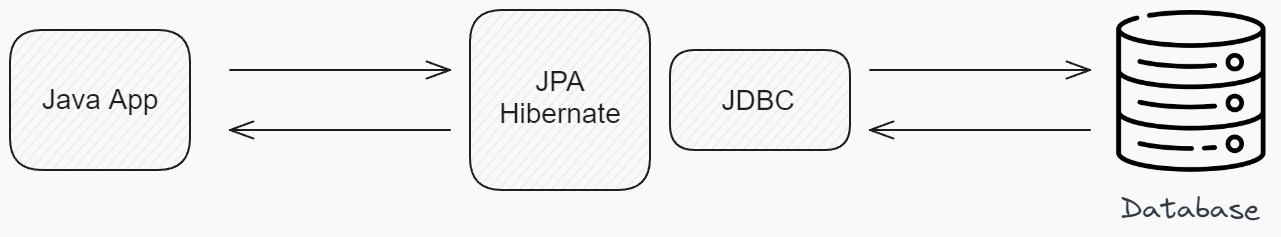
\includegraphics[width=1.0\textwidth]{images/jpa hibernate.png}
    \caption{Funzionamento di JPA con il framework ORM Hibernate.}
    \label{fig:jpa-hibernate}
\end{figure}

\subsection{Funzione crittografica di hash}
Una funzione crittografica di hash è un algoritmo che mappa dei dati di lunghezza arbitraria in una stringa binaria di dimensione fissa chiamata valore di hash, ma spesso chiamata digest.
Tale funzione di hash è progettata per essere unidirezionale (one-way), ovvero una funzione difficile da invertire: l'unico modo per ricreare i dati di input dall'output di una funzione di hash ideale, è quello di tentare una ricerca di forza bruta di possibili input per vedere se vi è un corrispondenza. \cite{funzioneCrittografica}

La funzione crittografica di hash ideale deve avere alcune proprietà fondamentali:
\begin{itemize}
    \item Deve identificare univocamente il messaggio, non è possibile che due messaggi differenti abbiano lo steso valore di hash;
    \item Deve essere deterministica, in modo che lo stesso messaggio si traduca sempre nello stesso hash;
    \item Il calcolo di un valore hash da un qualunque tipo di dato deve essere semplice e veloce;
    \item Deve essere molto difficile o quasi impossibile generare un messaggio dal suo valore hash se non provando tutti i messaggi possibili.
\end{itemize}
\newpage
\subsubsection{Bcrypt}
Bcrypt è una funzione crittografica di hash progettata per l'hashing delle password e l'archiviazione di queste ultime nel back-end delle applicazioni in modo tale da essere meno vulnerabile ad attacchi informatici.
Bcrypt esegue un processo di hasing complesso, durante il quale la password di un utente viene trasformata in un thread di caratteri a lunghezza fissa (Figura \ref{fig:bcrypt}).
Utilizza una funzione di hash unidirezionale, il che significa che una volta che la password è stata sottoposta ad hashing, non può essere ripristinata alla sua forma originale. Ogni volta che l'utente accede al proprio account, Bcrypt esegue nuovamente l'hasing della password e confronta il nuovo valore hash con la versione archiviata nella memoria del sistema per verificare se le password corrispondono. \cite{bcrypt}
\\
\begin{figure}[h]
    \centering
    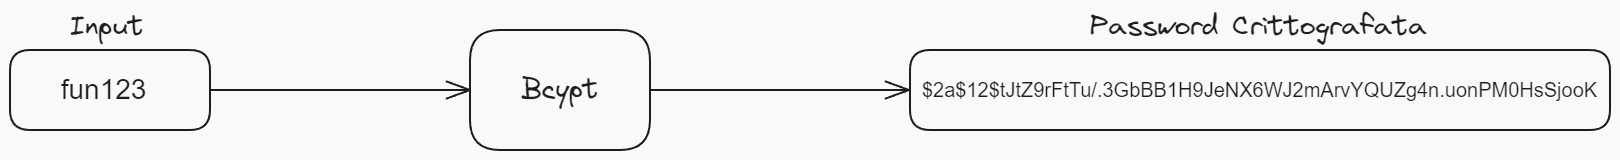
\includegraphics[width=1.0\textwidth]{images/Bcrypt.png}
    \caption{Funzionamento Bcrypt}
    \label{fig:bcrypt}
\end{figure}


\newpage
\section{Front-end: Tecnologie utilizzate}
Per l'implementazione del front-end ho utilizzato diverse tecnologie:
\begin{itemize}
    \item HTML
    \item CSS
    \item Bootstrap
    \item JavaScript
    \item Thymeleaf
\end{itemize}

\subsection{HTML}
HTML (Hypertext Markup Language) rappresenta la struttura portante delle pagine web: su questa struttura si possono aggiungere modifiche grafiche, grazie ai fogli di stile CSS ed elementi dinamici, grazie a JavaScript.
HTML è un linguaggio di markup gerarchico strutturato ad albero: esistono collegamenti gerarchici fra gli elementi, che rendono uno il genitore dell'altro ovvero il figlio.
HTML consente di descrivere semanticamente la struttura di un documento web attraverso tag, paragrafo, elenco, collegamento, citazione, o altri elementi.\cite{html}
\\
\begin{lstlisting}[language=html, basicstyle=\small, caption={Esempio di una pagina html}, captionpos=b]
<!DOCTYPE html>
<html lang="en">
<head>
    <meta charset="UTF-8">
    <meta name="viewport" content="width=device-width, initial-scale=1.0">
    <title>Document</title>
</head>
<body>

    <p>Hello World</p>
    
</body>
</html>
\end{lstlisting}
\newpage
\subsection{CSS}
CSS (Cascading Style Sheets) è un linguaggio usato per implementare lo stile di documenti scritti in un linguaggio di markup, come HTML e XML.
Con cascading in CSS si intende che i fogli di stile si applicano a cascata: quando un elemento è soggetto a diverse regole, tutte le regole sono valide, ma prevale sempre l'ultima regola. \cite{css}
Per applicare lo stile a un determinato elemento nella pagina HTML si utilizzano i selettori.

Esistono diversi tipi di selettori e vi sono delle priorità di applicazione di quest'ultimi (1 alta priorità, 6 bassa priorità):
\begin{enumerate}
    \item Dichiarazione con !important
    \item Inline style
    \item ID (\#) selector
    \item Class (.) selector, pseudo-class (:) selector
    \item Element selector
    \item Universal selector (*)
\end{enumerate}

\begin{lstlisting}[basicstyle=\small, caption={Esempio di utilizzo dei selettori usando CSS}, captionpos=b]
* {
  margin: 0;
  padding: 0;
  box-sizing: border-box;
}

p {
  font-family: sans-serif;
  color: black;
  font-size: 22px;
}

.author {
  font-style: italic;
  font-size: 18px;
}

#autor-text {
  font-size: 20px;
}

\end{lstlisting}

\subsection{Bootstrap}
Bootstrap è un framework di sviluppo web open source che permette la creazione di siti web responsive e mobile-first\footnote{Il termine Mobile First è una metodologia che promuove un modo di realizzare un’esperienza web pensata e creata nativamente per i display di dimensioni ridotte, come quelli degli smartphone e che viene progressivamente adattata e integrata per i display più grandi, come quelli dei computer desktop e delle TV.\cite{mobileFirst}}, facendo in modo che tutti gli elementi di un sito web funzionino in modo ottimale su tutte le dimensioni dello schermo.\cite{bootstrap}
Per fare ciò vengono utilizzati dei componenti, che sono recuperabili dalla documentazione.
\begin{lstlisting}[language=html, basicstyle=\small, caption={Esempio di un componente di Bootstrap (card)}, captionpos=b]
<div class="card" style="width: 18rem;">
  <img src="..." class="card-img-top" alt="...">
  <div class="card-body">
    <h5 class="card-title">Card title</h5>
    <p class="card-text">Some quick example text to build on the card title and make up the bulk of the card's content.</p>
    <a href="#" class="btn btn-primary">Go somewhere</a>
  </div>
</div>
\end{lstlisting}
\subsection{JavaScript}
JavaScript è un linguaggio di programmazione che viene utilizzato per di creare interazioni dinamiche quando si sviluppano pagine web, semplici e complesse, applicazioni, server. \cite{javascript}
JavaScript ha diversi vantaggi:
\begin{itemize}
    \item Semplicità: avere una struttura semplice rende JavaScript più facile da imparare e funziona più velocemente di altri linguaggi.
    \item Immediatezza: è eseguibile direttamente da un browser senza set-up aggiuntivi.
    \item Carico del server: operando lato client riduce le richieste inviate al server.
    \item Aggiornamenti: le community di sviluppatori aggiornano e creano nuovi framework e librerie.
\end{itemize}
\begin{lstlisting}[basicstyle=\small, caption={Esempio di script JavaScript}, captionpos=b]
document.querySelector(".btn-add").addEventListener("click", clear);

  function clear(e) {
    document.querySelector(".id-postit").value = "";
    document.querySelector(".titolo-postit").value = "";
    document.querySelector(".descrizione-postit").value = "";
  }
\end{lstlisting}
\newpage
\subsection{Thymeleaf}
Thymeleaf è un motore di template, una libreria scritta in Java, che consente agli sviluppatori di definire un modello di pagina HTML e in seguito riempirlo con i dati per generare la pagina finale.
Pertanto realizza una parte Model-View del Model-View-Controller.\cite{thymeleaf}
In particolar modo all'interno della classe Java avremo un oggetto di tipo Model, che fa da contenitore.\\
Ad esempio nella classe che fa da controller utilizziamo il model, e al suo interno possiamo inserire una lista di oggetti, a cui accederemo dalla pagina HTML per poi popolarla dinamicamente.\\
\begin{lstlisting}[language=java, basicstyle=\small, caption={Esempio di utilizzo del contenitore Model in un metodo del controller}, captionpos=b]
@RequestMapping(value = "/test")
public String showCheckbox(Model model) {
    boolean myBooleanVariable = false;
    model.addAttribute("myBooleanVariable", myBooleanVariable);
     
    return "sample-checkbox";
}
\end{lstlisting}

\begin{lstlisting}[language=html, basicstyle=\small, caption={Esempio di utilizzo di un attributo del Model all'interno della pagina HTML}, captionpos=b]
<input
 type="checkbox"
 name="myBooleanVariable"
 th:checked="${myBooleanVariable}"/>
\end{lstlisting}